% Consistency-novelty trade-off over the full common Ugi benchmark.
%
% PROVENANCE. Coordinates are transcribed from generated/common_ugi_benchmark_completed_rows.tex
% (mean and sample SD per 1,000 attempts, three seeds). They are inline rather than read from a CSV
% because generated/common_ugi_tradeoff.csv is emitted with a header and no rows: the producer
% declares these columns but writes no data. Point this figure at that CSV once the producer fills
% it, and delete the literals below. Until then these nine pairs must be rechecked whenever the
% benchmark artifact is reissued.
%
% x is reaction consistency, y is escape from the method's own component vocabulary. The y axis is
% method-relative by construction, which is exactly why the two families are drawn differently
% rather than as one population: for a method with no component vocabulary y is nearly all of x,
% so those points track the diagonal; for a catalogue method y is zero by
% Theorem~\ref{thm:catalogue-bound}. Comparing a filled point's y with an open point's y is not
% meaningful, and the caption says so.
\providecommand{\forgedatadir}{generated/}
\definecolor{tradeforge}{HTML}{55708A}
\definecolor{tradeother}{HTML}{8C8478}
\definecolor{tradeink}{HTML}{5C6474}

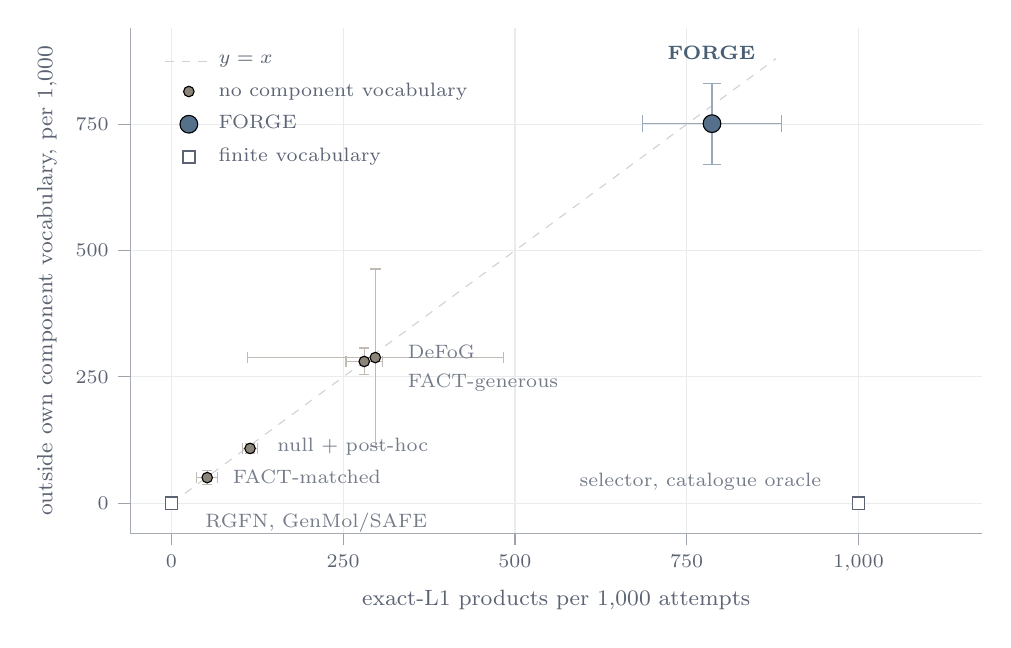
\begin{tikzpicture}
\begin{axis}[
  width=12.4cm, height=8.0cm,
  xlabel={exact-L1 products per 1{,}000 attempts},
  ylabel={outside own component vocabulary, per 1{,}000},
  xmin=-60, xmax=1180, ymin=-60, ymax=940,
  xtick={0,250,500,750,1000}, ytick={0,250,500,750},
  tick align=outside, tick style={color=tradeink!60, thin},
  every axis label/.style={font=\footnotesize, color=tradeink},
  tick label style={font=\scriptsize, color=tradeink},
  axis line style={color=tradeink!55, thin},
  axis x line*=bottom, axis y line*=left,
  grid=major, grid style={color=tradeink!13, thin},
  legend style={at={(0.03,0.97)}, anchor=north west, draw=none, fill=none,
                font=\scriptsize, text=tradeink, cells={anchor=west}, row sep=1.5pt},
  clip=false,
]
% y = x, explained in the caption rather than annotated across the plot
\addplot[draw=tradeink!30, dashed, thin] coordinates {(0,0) (880,880)};
\addlegendentry{$y=x$}
\addplot[only marks, mark=*, mark size=1.9pt, draw=none, fill=tradeother,
         error bars/.cd, x dir=both, x explicit, y dir=both, y explicit,
         error bar style={tradeother!55, thin}]
  coordinates {
    (0,0)         +- (0,0)
    (52.0,50.8)   +- (15.6,14.4)
    (114.4,108.5) +- (10.9,9.7)
    (280.6,280.6) +- (26.6,26.6)
    (296.7,288.3) +- (186.0,175.3)};
\addlegendentry{no component vocabulary}
\addplot[only marks, mark=*, mark size=3.2pt, draw=none, fill=tradeforge,
         error bars/.cd, x dir=both, x explicit, y dir=both, y explicit,
         error bar style={tradeforge!60, thin}]
  coordinates {(786.8,751.2) +- (100.8,80.2)};
\addlegendentry{FORGE}
\addplot[only marks, mark=square*, mark size=2.2pt, draw=tradeink, fill=white, line width=0.6pt]
  coordinates {(0,0) (1000,0) (1000,0)};
\addlegendentry{finite vocabulary}

% one consistent rule: label sits to the right of its point, and only where it fits
\node[font=\scriptsize, text=tradeink!85, anchor=west] at (axis cs:75,52)   {FACT-matched};
\node[font=\scriptsize, text=tradeink!85, anchor=west] at (axis cs:140,112) {null $+$ post-hoc};
\node[font=\scriptsize, text=tradeink!85, anchor=west] at (axis cs:330,300) {DeFoG};
\node[font=\scriptsize, text=tradeink!85, anchor=west] at (axis cs:330,238) {FACT-generous};
\node[font=\scriptsize, text=tradeink!85, anchor=west] at (axis cs:35,-38)  {RGFN, GenMol/SAFE};
\node[font=\scriptsize, text=tradeink!85, anchor=east] at (axis cs:960,42)
  {selector, catalogue oracle};
\node[font=\scriptsize, text=tradeforge!85!black, anchor=south] at (axis cs:786,858)
  {\textbf{FORGE}};
\end{axis}
\end{tikzpicture}
